\subsection*{Общая характеристика работы}

\newcommand{\actuality}{\underline{\textbf{Актуальность темы.}}}
\newcommand{\aim}{\underline{\textbf{Целью}}}
\newcommand{\tasks}{\underline{\textbf{задачи}}}
\newcommand{\defpositions}{\underline{\textbf{Основные положения, выносимые на~защиту:}}}
\newcommand{\novelty}{\underline{\textbf{Научная новизна:}}}
\newcommand{\influence}{\underline{\textbf{Практическая значимость}}}
\newcommand{\reliability}{\underline{\textbf{Достоверность}}}
\newcommand{\probation}{\underline{\textbf{Апробация работы.}}}
\newcommand{\contribution}{\underline{\textbf{Личный вклад.}}}
\newcommand{\publications}{\underline{\textbf{Публикации.}}}

\actuality\
Инструменты, предназначенные для~автоматического поиска дефектов в~программном коде, в~настоящее время получают всё большее распространение. Практика использования инструментов статического и динамического анализа закреплена в ряде методологий разработки безопасного программного обеспечения, таких как Microsoft SDL и TSP-Secure. Активное внедрение инструментов статического анализа объясняется практическим подтверждением их возможностей по обнаружению реальных дефектов в коде программ. 

Различные инструменты сильно различаются по характеристикам анализа: возможностям обнаружения дефектов (полноте), точности и скорости поиска. Задача точного и полного анализа программ на предмет поиска дефектов является алгоритмически неразрешимой, поскольку, согласно теореме Райса, невозможно для произвольной программы доказать её соответствие заданному нетривиальному свойству. В отношении задачи анализа программы это означает, что нельзя в общем случае найти все дефекты заданной программы по произвольно сформулированному критерию. Это приводит к необходимости применения различных ограничений и эвристик, что заставляет искать компромисс между достигаемыми характеристиками. Соответственно, различные методы статического анализа имеют различное соотношение между этими характеристиками.

Для анализа программных систем с высокими требованиями к качеству требуется высокая полнота анализа для обнаружения максимально возможного количества дефектов. Подобные анализаторы должны поддерживать межпроцедурный и межмодульный анализ программ. С увеличением структурной сложности системы возрастает время оценки корректности отчёта о дефекте и, соответственно, стоимость просмотра ложных срабатываний. Это значит, что при анализе сложных многокомпонентных программных систем также требуется высокая точность. Однако алгоритмы анализа с подобными характеристиками имеют экспоненциальную сложность относительно среднего количества операторов в программе, из-за чего они начали получать распространение лишь в последнее время. Множества состояний больших программных систем по определению имеют большую размерность, затрудняющую исследование или моделирование. Анализ больших графов выполнения, имеющихся в больших программных системах, с использованием данных алгоритмов требует длительного времени. Однако статический анализ имеет смысл применять постоянно в процессе разработки. Желательно также иметь возможность проводить анализ <<на лету>>, что также предъявляет повышенные требования к скорости анализа.

При интеграционном тестировании больших программных систем (содержащих большое количество компонент) возникают проблемы, связанные с резким ростом количества возможных путей выполнения программы. Разработанная модификация метода межпроцедурного анализа (МПА) позволяет снизить время, затрачиваемое на анализ путей выполнения программы, и увеличить покрытие графа выполнения в процессе анализа. Всё это приводит к повышению эффективности качества интеграционного тестирования.

Таким образом, повышение производительности межпроцедурного статического анализа имеет важную практическую значимость. Увеличение производительности позволяет осуществлять более полный и точный анализ крупных программ и программных систем, уменьшая время на поиск дефектов, а также позволяет ускорять анализ небольших программ.

Вопросы точного и полного, в т.~ч., межпроцедурного анализа рассматривались различными исследователями. Основополагающей в этой области может считаться работа J.~King (1976~г.), описывающая метод символьного выполнения программы. В~основе метода лежит идея разбиения входных данных на~классы эквивалентности в~зависимости от~встречаемых по пути выполнения условий. Два основных подхода к межпроцедурному анализу сформулированы Amir Pnueli и Micha Sharir. Подход к МПА на основе резюме был применён для смешанного анализа в работах Patrice Godefroid и впоследствии использован для реализации отдельных видов проверок в исследовательских работах Saswat Anand, Koushik Sen и George Necula, Jos\'{e} Miguel Rojas и Corina S. P\u{a}s\u{a}reanu. Попытка использовать резюме для моделирования циклов предпринималась в работах A.~Tsitovich и N.~Sharygina.

Однако данные работы посвящены поиску лишь ограниченного количества дефектов. Кроме того, в работах использован не статический, а смешанный и динамический анализ. В настоящее время требуется подход, который бы обеспечил возможность выполнения проверок произвольного вида, поскольку разработка одноцелевого анализатора является нецелесообразной. Наконец, упомянутые подходы слабо применимы для анализа больших объёмов программного кода из-за большого времени, затрачиваемого на анализ даже небольших программ. Промышленный статический анализатор должен быть многоцелевым, пригодным для решения различных классов задач и иметь возможность реализации широкого класса проверок. В рамках данной работы планировалось построение метода анализа крупных прикладных программных комплексов, разработанных с использованием языков C и C++, способного осуществлять анализ проектов масштаба ОС Android и ОС Tizen (порядка 5--20~млн. строк кода) за приемлемое время и обеспечивающего достаточное покрытие путей выполнения программы. Поэтому для разработки промышленного точного и полного статического анализатора требуется применение иных либо модифицированных подходов.

\aim\ данной работы является теоретическое обоснование и исследование подходов для модификации существующего метода межпроцедурного анализа, который будет использован для построения универсального анализатора кодов программ, разработанных с использованием языков C и C++, для дальнейшего встраивания в среду автоматического тестирования, с целью повышения эффективности анализа крупных прикладных программных комплексов. %построение метода анализа крупных прикладных программных комплексов, разработанных с использованием языков C и C++, способного осуществлять анализ проектов масштаба ОС Android и ОС Tizen \todo{(порядка 5--20~млн. строк кода)} за приемлемое время и обеспечивающего достаточное покрытие путей выполнения программы.

Для достижения указанной цели в диссертационной работе решаются следующие {\tasks}:
\begin{enumerate}
  \item Разработка модификации метода межпроцедурного анализа программ, пригодной для реализации в многоцелевом статическом анализаторе программного кода на языках C и C++ и позволяющей использовать различные виды проверок кода с целью поиска дефектов в нём.
  \item Разработка метода межмодульного анализа программ, реализованных с использованием языков C и C++, для повышения полноты анализа многокомпонентных систем.
  \item Реализация программного обеспечения (многоцелевой анализатор и его утилиты) на основе предложенных методов с целью его промышленного и коммерческого применения для поиска дефектов в исходном коде программных комплексов.
\end{enumerate}

\underline{\textbf{Объектом исследования}} являются методы, алгоритмы и инструменты статического анализа исходных кодов программ.

\underline{\textbf{Предметом исследования}} являются методы межпроцедурного и межмодульного анализа кодов программ, написанных на языке С и С++, их полнота, точность, производительность и масштабируемость.

\underline{\textbf{Соответствие паспорту научной специальности.}} Область исследования соответствует п.~1 <<Модели, методы и алгоритмы проектирования и анализа программ и программных систем, их эквивалентных преобразований, верификации и тестирования>> и п.~2 <<Языки программирования и системы программирования, семантика программ>>.

\underline{\textbf{Методы исследования}} основаны на теоретических положения теории компиляции и анализа программ, теории графов, конечных автоматов, теории множеств.

\novelty

Научная новизна диссертации определяется получением следующих результатов, которые выносятся на защиту:
\begin{enumerate}
  \item Формализованы функциональные требования к разрабатываемому в данной работе методу межпроцедурного анализа.
  \item Разработана модификация метода межпроцедурного анализа программ на основе резюме для метода символьного выполнения для программ, реализованных с использованием языков C и C++. Важными особенностями разработанного метода является поддержка проверок произвольного вида и их одновременного выполнения, а также поддержка модели памяти, используемой в языках C и C++, в том числе, с учётом арифметики указателей, наследования и выравнивания полей структур.
  \item Разработан алгоритм переименования областей памяти для трансляции имён переменных между различными функциями, использующий цепочки доступа. Данный алгоритм используется для установления соответствия между различными объектами, используемыми в функциях.
  \item Формализованы критерии достижимости и отсечения недостижимых ветвей выполнения программы с целью увеличения производительности анализатора при обработке больших графов выполнения (порядка $10^{11}$--$10^{12}$ узлов) в автоматическом режиме, а также устранения ложных срабатываний. Разработан алгоритм построения фрагментов графа выполнения, моделирующих вызов функции, с учётом ограничений на входные данные, известных на момент вызова функции. 
  \item Разработан метод межмодульного анализа программ, реализованных с использованием языков C и C++ для статического анализатора, использующего в качестве входных данных непосредственно исходный код программы. Использование промежуточного представления в виде синтаксического дерева программы позволяет производить анализ без потери информации о программе.
  \item Разработан алгоритм построения отчёта о дефекте при использовании предложенной модификации метода резюме для метода символьного выполнения. Данный метод позволяет строить информативный межпроцедурный отчёт, включающий показ переходов, выполнимых условий и представляющих интерес событий в процессе выполнения программы.
  \item Проведён сравнительный анализ метода МПА, использующего встраивание кода функции, и метода МПА, использующего резюме её эффектов. Результаты автоматического и ручного тестирования, проведённого для данных методов, показали значительное преимущество предложенного метода. Результаты также свидетельствуют об увеличении скорости поиска дефектов: то же самое количество уникальных дефектов можно находить за время, в 2--3 раза меньшее, в сравнении с методом встраивания. Ручная проверка части дефектов показала, что качество анализа при использовании метода резюме не уменьшается в сравнении с методом встраивания и составляет 80--84\%.


\end{enumerate}

\influence\ Разработаны методы анализа программ, применимые для проектов масштаба операционных систем и их наборов пользовательских приложений, реализованные в практически используемом анализаторе программного кода. Предложенные в диссертационной работе методы и алгоритмы позволяют проводить анализ программных систем объёмом порядка 5--20~млн. строк кода (или около $10^{11}$--$10^{12}$ узлов графа выполнения) в автоматизированном режиме. Данные методы и алгоритмы использованы для создания универсального анализатора кодов программ на языках C и C++. Разработан ряд проверяющих модулей с поддержкой предложенного метода межпроцедурного анализа, имеющих высокую и достаточную для практического применения точность анализа.

\underline{\textbf{Теоретическая значимость}} работы состоит в теоретическом обосновании преимущества метода резюме над методом встраивания в отношении полноты и производительности анализа. Формализованы и с помощью построенной математической модели временных затрат на межпроцедурный анализ показаны условия, при которых анализ с использованием метода резюме имеет преимущество перед методом встраивания. В работе показано, что при переходе от МПА с помощью метода встраивания к МПА с помощью метода резюме полнота анализа сохраняется. Показана возможность осуществления межмодульного анализа программ на языках C и C++ без применения компиляции их в промежуточный код.

\reliability\ полученных результатов обеспечивается экспериментальным подтверждением и последующей ручной проверкой отчётов анализатора при анализе исходного кода ОС Android версии 4.2.1. Ряд обнаруженных дефектов может быть найден с использованием других статических анализаторов, например, Coverity SAVE или Clang Static Analyzer (с режимом встраивания). Для тестирования был использован открытый исходный код, а разработанная экспериментальная система помещена в открытый доступ вместе с исходным кодом, что позволяет воспроизвести эксперименты независимо.

% \defpositions
% \begin{enumerate}
%   \item Модификация метода межпроцедурного анализа программ на основе резюме для метода символьного выполнения для программ, реализованных с использованием языков C и C++, с поддержкой проверок произвольного вида и их одновременного выполнения, а также поддержкой модели памяти, используемой в языках C и C++.
%   \item Алгоритм альфа-переименования областей памяти для трансляции имён переменных между различными функциями, использующий цепочки доступа.
%   \item Алгоритм построения фрагментов графа выполнения, моделирующих вызов функции, с учётом ограничений на входные данные, известных на момент вызова функции.
%   \item Метод межмодульного анализа программ, реализованных с использованием языков C и C++, использующий слияние синтаксических деревьев, позволяющий производить анализ без потери информации о программе.
%   \item Алгоритм построения отчёта о дефекте при использовании предложенной модификации метода резюме для метода символьного выполнения.
% \end{enumerate}

\underline{\textbf{Реализация и внедрение результатов работы.}} Результаты диссертационного исследования использованы при разработке программных средств поиска дефектов в составе комплекса статического анализа, используемой подразделениями Samsung Electronics, и используется для анализа исходного кода ПО различного назначения, в частности, мобильных приложений и операционных систем, телевизионного ПО, ПО медицинских систем, и может использоваться для других программных систем, включая настольные приложения и системы управления, с целью поиска потенциальных дефектов, что подтверждается актами о внедрении.

\probation\
Основные результаты работы докладывались~на:
\begin{enumerate}
 \item 10-й Международной Ершовской конференции <<Перспективы систем информатики>> (PSI 2015) (Казань, Россия, 2015)
 \item XII Международной научно-практической конференции <<Инновации на основе информационных и коммуникационных технологий>> (INFO-2015) (Сочи, Россия, 2015)
 \item Открытой конференции по компиляторным технологиям (Россия, Москва, 2015).
\end{enumerate}


\contribution\ Все выносимые на защиту результаты получены лично автором.

\publications\ Основные результаты по теме диссертации изложены в 4 печатных изданиях~\cite{summary-impl-mine,summary-intro-mine,summary-inter-unit-mine,info-2015},
3 из которых изданы в журналах, рекомендованных ВАК~\cite{summary-impl-mine,summary-intro-mine,summary-inter-unit-mine}, 
1~--- в тезисах докладов~\cite{info-2015}. В работах \cite{summary-impl-mine,summary-intro-mine,summary-inter-unit-mine} автору принадлежат теоретические модели, обзорные разделы, описание элементов разработанных методов, а также результаты экспериментального тестирования разработанного в рамках работы ПО.

\textbf{Объем и структура работы.} Диссертация состоит из введения, четырёх глав и заключения. Полный объём диссертации составляет 131 страницу с 18 рисунками и 12 таблицами. Список литературы содержит 71 наименование.


 % Характеристика работы по структуре во введении и в автореферате не отличается (ГОСТ Р 7.0.11, пункты 5.3.1 и 9.2.1), потому её загружаем из одного и того же внешнего файла, предварительно задав форму выделения некоторым параметрам

%Диссертационная работа была выполнена при поддержке грантов ...

%\underline{\textbf{Объем и структура работы.}} Диссертация состоит из~введения, четырех глав, заключения и~приложения. Полный объем диссертации \textbf{ХХХ}~страниц текста с~\textbf{ХХ}~рисунками и~5~таблицами. Список литературы содержит \textbf{ХХX}~наименование.

%\newpage
\subsection*{Содержание работы}
Во \underline{\textbf{введении}} обосновывается актуальность исследований, проводимых в рамках данной диссертационной работы, приводится обзор научной литературы по изучаемой проблеме, формулируется цель, ставятся задачи работы, сформулированы научная новизна и практическая значимость представляемой работы, приведены сведения об апробации работы и публикациях.

\underline{\textbf{Первая глава}} посвящена анализу моделей и средств, применяемых для статического анализа компьютерных программ с различной точностью и полнотой. Приведены результаты исследований существующих подходов к анализу программ с целью проверки соответствия их задаваемым требованиям. Проведено исследование особенностей точных и полных методов анализа программного кода. Выполнен анализ различных модельных представлений программ и возможностей их использования для поиска дефектов в исходном коде программ.

Рассмотрены основные проблемы, возникающие при использовании методов точного анализа программ, требующих получения наибольшего количества информации об операторах программы и влияние их выполнение на состояние программы для учёта при моделировании. Обосновано применение метода символьного выполнения, подразумевающего разбиение множества входных данных на классы эквивалентности в зависимости от условий, встречаемых на пути выполнения программы. Показано, что одним из основным препятствий для использования метода символьного выполнения является резкое снижение производительности при использовании межпроцедурного анализа. Показана необходимость использования контекстно-чувствительного межпроцедурного анализа для повышения его точности.

Рассмотрены исследования в области межпроцедурного анализа. В качестве наиболее перспективного был выбран метод межпроцедурного анализа с использованием резюме, поскольку он позволяет сохранять все виды чувствительностей анализа.
% и, в особенности, метод символьного выполнения как один из наиболее актуальных и используемых на практике. Рассмотрены основные проблемы, возникающие при использовании данного метода, и методы их решения. Представлены и проанализированы работы, посвящённые улучшениям метода символьного выполнения, в т.~ч. наиболее близкие к тематике работы.


Во \underline{\textbf{второй главе}} рассмотрен и подробно описан метод межпроцедурного анализа программ с использованием резюме для метода символьного выполнения. Произведена оценка потенциальной производительности при использовании данного метода. Показано, что при использовании данного метода можно получить существенный прирост производительности в сравнении с методом встраивания.

При~встраивании функций вызываемая функция анализируется каждый раз при~её вызове. При~этом в~случае контекстно-чувствительного анализа функция анализируется не~полностью, поскольку анализируются лишь те пути выполнения, которые являются достижимыми при~контексте на~момент вызова. При~использовании подхода, основанного на~резюме, вызываемая функция анализируется один раз, но полностью. Однократный характер также носят затраты, связанные с~составлением резюме функции. Применение резюме выполняется в~каждой точке вызова функции. В результате оценки затрат на различные этапы анализа при использовании обоих методов, получаем, что для~получения ускорения необходимо выполнение соотношения $t_{\text{ср. применения}} <  t_{\text{ср.}}$, где $t_{\text{ср. применения}}$~--- среднее время применения резюме функции, а $t_{\text{ср.}}$~--- среднее время, затрачиваемое на анализ встраиваемых функции.

Резюме функции составляется как композиция эффектов операторов программы на каждой из ветвей выполнения. Разработанный алгоритм метода межпроцедурного анализа с помощью резюме для метода символьного выполнения выглядит следующим образом:

\begin{enumerate}
 \item[Шаг 1.] Провести внутрипроцедурный анализ вызываемой функции методом символьного выполнения. В результате этого анализа получаем граф выполнения вызываемой функции.
 \item[Шаг 2.] Для каждого конечного узла графа выполнения функции осуществить сбор эффектов, оказываемых на состояние программы при выполнении данной ветви выполнения. Полученным результатом является набор ветвей резюме.
 \item[Шаг 3.] В каждой точке вызова проанализированной функции для каждой ветви резюме создать новый узел графа выполнения (узел применения резюме) и соединить эти узлы с узлом, соответствующим вызову функции (узлом вызова). Состояние программы в каждой точке применения резюме есть композиция состояния программы в узле вызова и функции, описываемой соответствующей ветвью резюме.
\end{enumerate}

Каждый оператор при своём выполнении производит эффект, заключающийся в изменении состояния программы. В случае анализа речь идёт о моделировании эффектов операторов. Сократить время анализа при использовании резюме в сравнении со встраиванием можно получить за счёт отсутствия необходимости затрачивать время на анализ эффектов, действия которых локальны или не учитываются при дальнейшем анализе из-за особенностей анализатора. Время, затрачиваемое на применение резюме, по-прежнему не будет превышать время, требуемое на анализ вызова функции методом встраивания. Это объясняется тем, что набор эффектов, получаемых в результате применения резюме, включается строго или совпадает с набором эффектов, моделируемых при анализе методом встраивания. В данной работе рассмотрен следующий набор эффектов, оказывающих влияние на состояние анализируемой программы в процессе её выполнения.

\begin{enumerate}[leftmargin=1em]
 \item Принятие решений о выборе пути выполнения. Выбор пути выполнения сопровождается наложением ограничений на символьные значения, относительно которых принимается решение о выборе пути. Эти ограничения учитываются при \textit{анализе достижимости} ветвей выполнения программы.
 
 \item Модификация регионов памяти с нелокальной областью видимости.
 
 \item Инвалидация регионов памяти, то есть пометка некоторых регионов как изменивших значение на неизвестное.
 
 \item Возврат вызываемой функцией некоторого значения. Это значение связывается с выражением вызова функции.
 
 \item Пометки проверяющих модулей, в т.~ч. пометки состояния программы и пометки отложенных проверок.
 
\end{enumerate}

Поскольку проверяющие модули самостоятельно отвечают за свои данные, логику обработки резюме для проверок имеет смысл включать непосредственно в логику работы этих модулей. Данное решение позволяет реализовывать одновременную работу различных проверок в процессе моделирования выполнения программы. Недостаток данного решения заключается в том, что оно требует дополнительной поддержки со стороны разработчиков проверяющих модулей.

Таким образом, в результате сбора резюме получается набор \textit{предусловий}, при которых достижима данная ветвь выполнения функции, и \textit{постусловий}, которые являются эффектами выполнения данной ветви функции.

Одним из результатов сбора резюме являются пары <<регион памяти~--- символьное значение>>. В результате актуализации символьных значений из резюме могут получиться символьные значения, имеющие диапазон конкретных значений, отличный от диапазона этого символьного значения в контексте вызывающей функции. Это является следствием того, что при моделировании условий внутри вызываемой функции может произойти разделение входных данных функции (аргументов и внешних переменных) на классы эквивалентности. Новое множество конкретных значений вычисляется следующим образом. Введём следующие обозначения:

 $n$ – количество ветвей выполнения в резюме вызываемой функции,
 
 $s_{ij}$ – символьное значение с номером $j$ в $i$-ой ветви,
 
 $r_{\text{вх.}\ ij}$ – множество значений $s_{ij}$ в контексте вызывающей функции,
 
 $r_{\text{рез.}\ ij}$ – множество значений $s_{ij}$ в контексте вызываемой функции,
 
 $state_{\text{входное}}$~--- состояние программы в контексте вызывающей функции в точке непосредственно перед вызовом функции,

 $state_{\text{выходное}}$~--- состояние программы после вызова функции (после применения резюме).

Тогда при применении резюме $\forall i, \forall j:\ r_{\text{вых.}\ ij} =  r_{\text{вх.}\ ij} \cap r_{\text{резюме}\ ij}$, то есть результирующее множество является пересечением множеств входных конкретных значений символического значения и множества конкретных значений символического значения из применяемой ветви резюме.

В случае, если результирующее множество конкретных значений является пустым хотя бы для одного символического значения, то данная ветвь выполнения является недостижимой и не принимается в дальнейшее рассмотрение, что может быть выражено формулой:
\begin{equation*}
 \label{empty_set}
 (\exists i, j: r_{\text{вх.}\ ij} \cap r_{\text{рез.}\ ij} = \varnothing)  \Rightarrow (state_{\text{входное}} \nrightarrow state_{\text{выходное}})
\end{equation*}

Поскольку при передаче аргумента в функцию не по значению его значение может измениться, необходимо различать входное значение региона до его изменения в функции и выходное значение. Для получения информации о разбиении данных на классы эквивалентности отслеживается событие потери активности и определяем диапазон возможных значений символа, связанного с данным регионом, в данной ветви выполнения. При этом первое событие потери активности соответствует диапазону входных значений, а последнее соответствует диапазону выходных значений. Сбор выходных значений также бывает необходимо проводить по окончании пути выполнения функции.

Под инвалидацией региона памяти понимается связывание с данным регионом нового символа, без наложенных на него ограничений, т.~е. способного принимать произвольные значения. Поскольку символьные значения, связанные с регионами памяти, обрабатываются при завершающем проходе по хранилищу, а значения регионов, актуальные до инвалидации, обрабатываются по событию потери активности, непосредственно предшествующему событию связывания нового значения, инвалидация обрабатывается автоматически, и дополнительных действий для обработки инвалидаций регионов памяти не требуется.

Для обработки возврата функцией значения результирующее символьное значение сохраняется в резюме целиком, а ограничения, накладываемые на него и на его части, обрабатываются отдельно.

За хранение данных проверок проверяющие модули отвечают самостоятельно. Основными видами данных проверок является отметка отложенной проверки и данные состояния проверки. Отложенные проверки используются для выдачи предупреждений в тех ситуациях, когда из-за отсутствия данных о контексте вызова невозможно однозначно утверждать наличие дефекта или его отсутствие. Данные состояния используются для построения нового состояния проверки при применении резюме. 

В результате сбора резюме получается некоторое множество регионов памяти, с которыми связаны некоторые символьные значения. Кроме того, регионы памяти сами могут входить в символьные значения как их составная часть. Однако, полученные регионы памяти адресуются в контексте объявлений имён внутри функции. В контексте вызывающей функции эти регионы могут иметь уже другое значение, то есть регионы, используемые внутри функции, являются относительными по отношению к вызывающей функции. Так, например, в контексте вызываемого метода класса регион памяти, связанный с указателем \texttt{this}, будет адресоваться безотносительно какого-либо объекта, а в контексте вызывающей функции этот регион будет регионом объекта, метод которого вызывается. Кроме того, с регионом памяти в контексте вызываемой функции может быть связано значение, не имеющее в своей основе регион аргумента, например, константа. Всё это означает, что для корректного применения резюме необходимо производить актуализацию символьных значений, то есть их перевод из контекста имён и значений вызываемой функции в контекст имён и значений вызывающей функции.

Идея актуализации заключается в следующем. Пусть имеется символьное значение. В его состав могут входить символы, регионы памяти и константы. Они, согласно модели анализатора, образуют дерево. Непосредственно актуализации подвергаются только регионы памяти. Таким образом, в символьном значении происходит подмена регионов памяти, содержащихся в нём, на актуализированные. Затем, если это возможно, символы полученного символьного выражения вычисляются в константы, заменяя исходные поддеревья. Данная процедура актуализации реализуется с помощью следующего алгоритма.

\begin{enumerate}
 \item[Шаг 1.] Для всех регионов памяти, содержащихся в символьном значении, создать новый регион, являющийся актуализацией данного региона и заменить в символьном значении исходный регион актуализированным регионом.
 \item[Шаг 2.] Для всех символов, содержащихся в символьном значении, полученном на шаге 1, проверить, не вычисляется ли символ в константу, и, если символ вычисляется в константу, заменить данный символ вычисленной константой.
\end{enumerate}

Схемы применения резюме, описанные выше, затрагивают отсечение недостижимых ветвей выполнения программы и уточнение множества конкретных значений для символьных значений. Однако для того, чтобы анализатор имел возможность выполнять проверки при вызове функции, необходима доработка проверяющих модулей. Для получения проверяющими модулями возможностей анализа при использовании резюме вводятся две дополнительных функции обратного вызова. Первая из них (названная \texttt{evalSummaryPopulate}) вызывается для сбора резюме проверяющим модулем, вторая (названная \texttt{evalSummaryApply}) вызывается при применении резюме.

Проверяющий модуль, подписанный на событие \texttt{SummaryPopulate}, должен сохранить информацию, которая может понадобиться для обновления состояния или для выполнения отложенной проверки. Информация, содержащая в резюме, не освобождается до окончания работы анализатора, поэтому проверяющий модуль может использовать произвольный формат хранения данных, отвечающий задаче проверки. Обычно для каждой проверки, проводимой модулем, в GDM помещаются две дополнительных записи, которые затем будут использоваться для заполнения резюме~--- для обновления состояния и для отложенной проверки.

При обработке события \texttt{SummaryApply} проверяющий модуль должен произвести обновление состояния в соответствии с информацией, хранящейся в выбранной ветви резюме. Так, если при выполнении вызова функции дескриптор был закрыт, он должен быть помечен как закрытый в состоянии вызывающей функции. Если же в контексте вызывающей функции уже известно, что дескриптор закрыт, то отложенная проверка должна выдать предупреждение.

 Введём обозначения:

\begin {itemize}
 \item $N$~--- количество узлов графа выполнения;
 \item $S_i$~--- содержимое памяти в $i$-м узле графа выполнения;
 \item $|S_i|$~--- количество элементов (записей) в содержимом памяти $i$-го узла графа выполнения;
 \item $E_i$~--- множество активных выражений в $i$-м узле графа;
 \item $|E_i|$~--- количество элементов (записей) во множестве активных выражений в $i$-м узле графа;
 \item $C_{ik}$~--- множество элементов $k$-й проверки в $i$-м узле графа. В это множество входит также множество ограничений ($C_0$);
 \item $M$~--- количество проверок,
 \item $D$~--- глубина стека вызовов (вложенность вызова);
 \item $NParams_d$~--- количество аргументов $d$-й функции в стеке вызовов
\end {itemize}

Пусть функция анализируется относительно состояния $State'$ на момент вызова, которое имеет в модели памяти и в множестве активных выражений некоторые множества записей $S'$ и $E'$ соответственно. Аналогичные множества записей $C'_k$ будут существовать в структурах данных проверок.

В работе показано, что асимптотическая временная сложность анализа графа выполнения вызываемой функции при использовании метода встраивания будет следующей:
\begin{equation}
\label{eq:inlining-full}
\begin{split}
 T(N) = \Theta \left( a_E \sum_{i=0}^N \log \left(\sum_{d = 0}^D |E'_d| + |E_i| \right) + \right. \\
 + a_S \sum_{i=0}^N \log \left(\sum_{d = 0}^D \left(|S'_d| + NParams_d \right) + |S_i|\right)+ \\
 + \left.a_C \sum_{i=0}^N \sum_{k=0}^M  \log \left(\sum_{d = 0}^D |C'_d|  + |C_{ik}|  \right) \right),
 \end{split}
\end{equation}

В работе также показано, что при использовании разработанного метода, использующего резюме функции,  сложность анализа в наихудшем случае $O(N)$ может быть представлена следующей зависимостью:

\begin{equation}
\label{eq:summary-apply}
\begin{split}
 T(N) = O \left( a_S \sum_{i=0}^N \log \left(|S'| + |S_i|\right) +  a_C \sum_{i=0}^N \sum_{k=0}^M  \log \left(|C'|  + |C_{ik}|  \right) \right).
 \end{split}
\end{equation}

Эти соотношения позволяют заключить, что разрабатываемый метод МПА имеет алгоритмическую сложность меньшую, чем метод встраивания. Основным источником прироста производительности, как следует из формул, является отсутствие моделирования операторов языка.

Интерес представляет сравнение двух методов обработки данных проверяющими модулями. Определим два вида проверок формально. Проверку при использовании метода встраивания определим следующим образом. Пусть имеется граф выполнения программы в виде дерева. Алгоритм поиска осуществляет обход дерева от корня к листу по пути $w$ без возврата, собирая ограничения, наложенные на входные данные, и отслеживая изменение состояния программы в каждом узле графа выполнения. Алгоритм поиска выдаёт срабатывание в случае обнаружения нарушения заданного для него условия корректности состояния программы в заданной точке, таким образом представляя дефект конъюнкцией $pre_w \wedge node_w$, т.~е. отображением множества значений входных данных функции на узел графа выполнения, состояние которого нарушает условие корректности программы.

Проверку при использовании метода резюме определим как проверку при использовании метода встраивания для функции верхнего уровня и отложенную проверку при использовании межпроцедурного вызова. Под отложенной проверкой понимается дополнительная проверка всех узлов графа выполнения вызываемой функции в узле применения резюме с актуализацией состояния в данных узлах с учётом контекста вызова и актуализированных ограничений на момент выхода из вызываемой функции. Отложенная проверка и обычная проверка производятся с использованием одного критерия корректности состояния программы.

В данной главе приведены и доказаны два утверждения. Они показывают, что в случае идеального анализатора метод резюме для символьного выполнения при использовании различных видов и последовательностей проверок не уступает в полноте анализа методу встраивания. Это важное заключение подтверждает перспективность выбранного для модификации метода МПА.

\textbf{Утверждение 1}. Если при использовании проверки с помощью метода встраивания результатом проверки является предупреждение, выданное в некотором узле графа выполнения программы, то при использовании метода резюме для той же функции верхнего уровня и того же набора вызываемых функций результатом проверки методом резюме также является предупреждение, выданное в узле графа выполнения вызывающей функции или в одном из узлов графов выполнения вызываемых функций.

\textbf{Утверждение 2}. При использовании отложенной проверки в конце анализа функции верхнего уровня при использовании МПА методом встраивания и МПА методом резюме множества срабатываний совпадают.

Важным элементом работы статического анализатора является построение отчёта. При анализе программы методом анализа её путей выполнения необходимо выполнять построение подробного отчёта, однозначно указывающего условия, при которых проявляется дефект, и соответствующий им путь выполнения. При применении метода резюме, в отличие от метода встраивания, возникает проблема потери информации о части пути, проходимом внутри вызываемой функции, поскольку явного построения поддеревьев графа выполнения программы более не происходит. Для построения отчёта  при межпроцедурном анализе методом резюме в настоящей работе предлагается сохранять в узлах применения резюме ссылки на соответствующий лист графа выполнения вызываемой функции и ссылки на узлы отложенной проверки (для проверяющих модулей).

В \underline{\textbf{третьей главе}} приводится описание разработанного метода межмодульного анализа программ с использованием непосредственно исходного кода, а также рассматриваются проблемы, возникающие при межмодульного анализе больших программных комплексов, и методы их решения. Межмодульный анализ, в отличие от внутримодульного, позволяет использовать определения функций и структур данных в любой единице трансляции проекта, а не только в текущей. Это позволяет находить различные классы дефектов программного кода, не обнаруживаемые при внутримодульном анализе или труднообнаружимые с его помощью, в т.~ч. ошибки интеграции модулей и подсистем программы или программного комплекса, некорректное использование программных интерфейсов. Межмодульный анализ становится особенно полезным для языков программирования, допускающих раздельную компиляцию исходных файлов (в т.ч. C/C++), поскольку в этом случае информация о программе, содержащаяся в одном исходном файле, становится ограниченной и затрагивает лишь малую часть программного проекта.

В результате проведённого исследования была разработана архитектура анализатора, позволяющего производить межмодульный анализ программы на языках C и C++ и использующего для анализа непосредственно исходный код программы. Разработанная схема межмодульного анализа интересна тем, что позволяет использовать различные алгоритмы межпроцедурного анализа, т.~е. как анализ методом встраивания, так и анализ методом резюме, без дополнительных модификаций как самого алгоритма межпроцедурного анализа, так и проверяющих модулей. Последовательность операций, выполняемых при межмодульном анализе, представлена на рисунке \ref{xtu-idef0}.

\begin{figure}[h]
 \label{}
 \centering
 \includegraphics[width=\linewidth]{xtu-idef0-3}
 \caption{Функциональная модель межмодульного анализа}\label{xtu-idef0}
\end{figure}


Единицей анализа в анализаторах исходных кодов обычно является единица трансляции, представляющая собой препроцессированный файл исходного кода. Однако для выполнения межмодульного анализа недостаточно информации, содержащейся в одной единице трансляции. Необходимо знать расположение определений функций, необходимых для анализа других функций. Кроме того, необходимо знать не только имя и путь к файлу, где располагается определение функции. Для корректного построения импортируемого синтаксического дерева файла с исходным текстом необходимо знать, например, аргументы команды сборки файла, расположение включаемых файлов, использовавшихся для построения, и некоторую другую информацию.

В данной работе реализован трёхфазный анализ с сохранением промежуточных результатов в файлах в директории проекта. На \textit{фазе сборки} собирается информацию об анализируемых единицах трансляции. Для этого производится перехват вызовов компилятора во время построения проекта. Для каждой обнаруженной команды записываются сигнатуры экспортируемых определений функций данной единицы трансляции и сигнатуры используемых (импортируемых) функций, определения которых в данном модуле трансляции недоступны. Для каждой обнаруженной функции строится локальный граф вызовов. На фазе сборки также создаются образы синтаксических деревьев всех модулей трансляции. Определения функций различаются по тройке <путь к файлу, сигнатура функции, целевая архитектура>, которая используется для выбора нужного определения функции и его импорта.

На \textit{фазе предобработки данных} обрабатывается служебная информации, собранная на фазе сборки. На этой фазе строится соответствие между сигнатурами импортируемых функций и строится глобальный граф вызовов с использованием локальных графов вызовов, сгенерированных на предыдущей фазе. Выполняется топологическая сортировка построенного глобального графа вызовов. При этом сортируются не сами функции, а файлы, их содержащие, поскольку анализ отдельных функций из файла означает многократную загрузку одних и тех же файлов.

На вход \textit{фазы анализа} поступает упорядоченный набор файлов для анализа. Все эти файлы добавляются в очередь анализа в порядке следования, и полученная очередь начинает обрабатываться пулом рабочих процессов анализатора. Данная схема позволяет осуществлять анализ с очень высокой степенью параллелизма, т.~к. различные процессы не используют разделяемых ресурсов, и производительность системы линейно растёт с увеличением количества процессоров. Каждый процесс анализатора из пула анализирует свою единицу трансляции, подгружая отсутствующие определения функций и структур данных по мере необходимости.

В данной разработке был реализован межмодульный анализ с использованием слияния синтаксических деревьев анализируемых единиц трансляции. Когда анализатор обнаруживает функцию с недоступным определением, производится поиск сигнатуры этой функции в сгенерированном отображении и, если сигнатура функции была найдена, загружается синтаксическое дерево файла, содержащего определение этой функции. Затем эта функция импортируется в основное синтаксическое дерево вместе с необходимыми определениями и объявлениями.

Задача импорта фрагментов синтаксического дерева обычно решается с помощью поиска определения в целевом AST. Если аналогичное определение (или объявление) не найдено, оно создаётся в целевом AST с использованием специального интерфейса. Новый фрагмент является рекурсивной копией исходного, но в процессе импорта зависимостей также производится поиск в целевом контексте, и не все части нового фрагмента синтаксического дерева обязательно являются созданными заново, если они уже присутствуют в целевом AST.

Этот раздел посвящён различным проблемам при импорте и их возможным методам решения. Первой проводимой операцией при импорте объявления из исходного контекста является поиск похожего объявления в целевом синтаксическом дереве. Этот поиск часто включает в себя рекурсивный обход вложенных объявлений для определения, являются ли два объявления структурно эквивалентными. В данной работе, однако, испытан ряд простых и легковесных эвристик, ускоряющих поиск за счёт частичного отказа от рекурсивного обхода. Рекурсивная проверка структурной эквивалентности выполняется только в случае, если эти эвристики не смогли однозначно показать различие или эквивалентность. Во-первых, если два объявления имеют различные разновидности, они, очевидно, не являются структурно эквивалентными. Во-вторых, если два объявления имеют различные имена, их можно определённо считать различными без дальнейшего просмотра. В-третьих, в большинстве случаев объявления с совпадающими местоположениями в исходных файлах являются эквивалентными, за исключением специализируемых шаблонов. Основная проблема этой эвристики заключается в обработке конфликтующих объявлений.

Если эвристика не сработала, происходит возврат к рекурсивному обходу, что является одной из основных проблем импорта. Для импорта объявления необходимо сначала импортировать его контекст объявления. Этот контекст, в свою очередь, может иметь большое количество вложенных объявлений и их зависимостей. В результате происходит массовый рекурсивный импорт зависимостей как самого объявления, так и его контекста. Иногда встречаются циклические зависимости, образуемые опережающими объявлениями. Это вызывает необходимость переупорядочения  полей структур после того, как определение структуры было полностью импортировано, в соответствии с их порядком в импортируемой структуре, для сохранения порядка объявлений и модели раскладки в памяти.

Код, успешно прошедший компиляцию и компоновку, может содержать несовместимые друг с другом определения. Проблема при наличии конфликтующих определений заключается в выборе стратегии поведения анализатора. Первой стратегией может стать выдача предупреждения об обнаружении конфликтующего определения с последующим завершением работы анализатора или пропуском импорта данного определения. Несмотря на логичность такого подхода, данная стратегия имеет недостаток: разработанный программный код, возможно, всё равно имеет смысл проанализировать, поскольку его работоспособность, как правило, проверяется при тестировании. Вторая стратегия заключается в разрешении конфликтов между определениями. Её недостаток заключается в том, что у анализатора может не быть данных о программе для корректного разрешения конфликта.


В \underline{\textbf{четвертой главе}} приведены результаты и методики тестирования программного обеспечения, реализующего разработанные методы межпроцедурного и межмодульного анализа. В данной главе проводится сравнение двух методов МПА~--- встраивания и резюме по трём характеристикам:
\begin{itemize}[leftmargin=1em]
 \item \textit{производительности анализа}, которая определяется временем, затраченным на анализ программного кода, предоставленного для обработки статическим анализатором;
 \item \textit{точности анализа}, которая представляет собой отношение количества корректных срабатываний анализатора к их общему количеству;
 \item \textit{полноте анализа}, которую будем оценивать количеством обработанных узлов графа выполнения программы.
\end{itemize}

Использование межмодульного анализа резко увеличивает количество  путей программы, требующих статического анализа. Следовательно, при сравнении производительности и точности межпроцедурного анализа методом встраивания и разработанного автором метода резюме необходимо оценить как внутримодульный, так и межмодульный анализ.

В данной главе приводятся результаты тестирования разработанных методов. В качестве тестовой системы были выбраны пакеты пользовательских программ и библиотек из состава ОС Android 4.2.1. В качестве тестовой базы были взяты пакеты ОС Android версии 4.2.1. Результаты тестирования представлены на рис. \ref{img:nodes} и \ref{img:defects} в виде графиков.


\begin{figure}[ht]
  \begin{minipage}[ht]{0.49\linewidth}
    \center{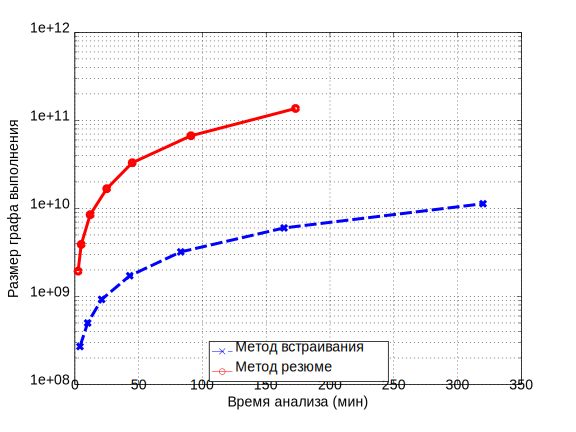
\includegraphics[width=\linewidth]{single-nodes} \\ а)}
  \end{minipage}
  \hfill
  \begin{minipage}[ht]{0.49\linewidth}
    \center{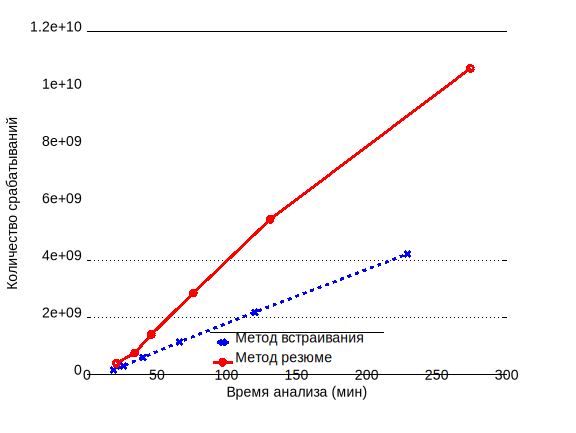
\includegraphics[width=\linewidth]{xtu-nodes} \\ б)}
  \end{minipage}
  \caption{Количество анализируемых узлов графа при внутримодульном (а) и межмодульном анализе (б) для методов встраивания и резюме}
  \label{img:nodes}  
\end{figure}

\begin{figure}[ht]
  \begin{minipage}[ht]{0.49\linewidth}
    \center{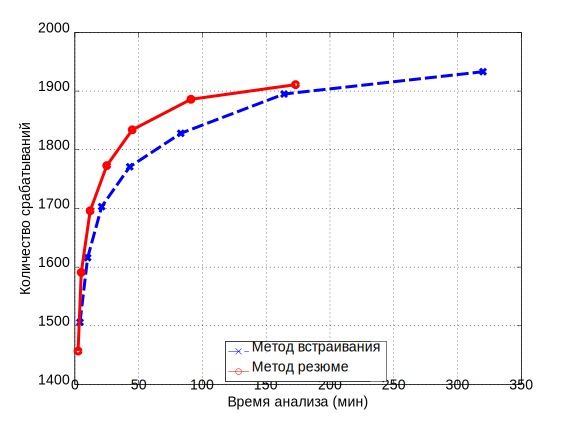
\includegraphics[width=\linewidth]{single-unique} \\ а)}
  \end{minipage}
  \hfill
  \begin{minipage}[ht]{0.49\linewidth}
    \center{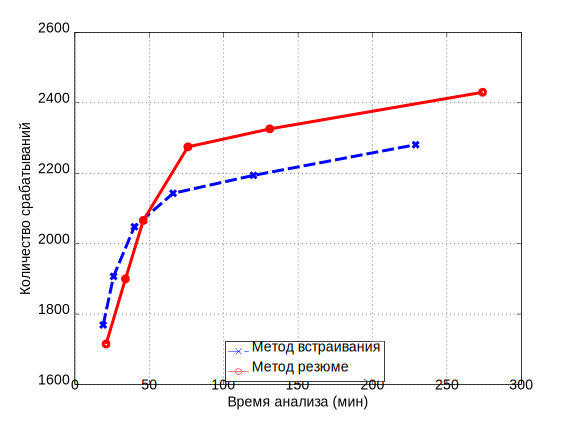
\includegraphics[width=\linewidth]{xtu-unique} \\ б)}
  \end{minipage}
  \caption{Количество выдаваемых отчётов при внутримодульном (а) и межмодульном анализе (б) для методов встраивания и резюме}
  \label{img:defects}  
\end{figure}

Согласно данным измерений, количество анализируемых в единицу времени операторов программы увеличилось до 10 раз. Результаты также свидетельствуют об увеличении скорости поиска дефектов: то же самое количество уникальных дефектов можно находить за время, в 2--3 раза меньшее, в сравнении с методом встраивания. Аналогичные выводы можно сделать по результатам межмодульного анализа системы. Ручная проверка части дефектов показала, что качество анализа при использовании метода резюме не уменьшается в сравнении с методом встраивания и составляет от 80\% до 84\% в зависимости от настроек глубины анализа.

В \underline{\textbf{заключении}} диссертации приведены основные результаты работы, а также приведены направления дальнейших исследований.% Одним из наиболее вероятных направлений исследования представляется дальнейшая работа над межмодульным анализом в отношении повторного использования резюме функции, что потенциально может заметно сократить время анализа. Кроме того, описанный метод резюме можно адаптировать для моделирования операторов циклов, что также может стать одним из направлений работы.

\underline{\textbf{Основные результаты}} настоящей диссертационной работы заключаются в разработке метода точного межпроцедурного анализа, пригодного для программ и программных комплексов большого объёма, и его реализации в составе законченного программного средства, предназначенного для поиска дефектов в исходном коде программ.
\begin{enumerate}[leftmargin=1em]
  \item Разработан метод межпроцедурного анализа программ на основе резюме для метода символьного выполнения для программ, реализованных с использованием языков C и C++. Данный метод подходит для реализации различных классов проверок, и на его основе была реализована поддержка межпроцедурного анализа для проверок различного назначения.
  \item Разработан метод межмодульного анализа программ, реализованных на языках C и C++, для статического анализатора, использующего в качестве входных данных непосредственно исходный код программы.
  \item Разработан метод построения отчёта о дефекте при использовании метода резюме для метода символьного выполнения.
  \item Для экспериментального подтверждения эффективности разработанные методы реализованы для использования в составе статического анализатора Clang Static Analyzer. Произведено тестирование разработанных методов на реальных программных проектах~--- пакетах пользовательского окружения ОС Android. Результаты тестирования подтвердили значительный прирост производительности анализа, покрытия путей выполнения и скорости поиска дефектов. Реализованное на основе разработанных методов ПО позволяет производить обработку больших графов выполнения (порядка $10^{11}$--$10^{12}$ узлов) программных комплексов объёмом 5--20 млн. строк кода в автоматическом режиме. Результаты также свидетельствуют об увеличении скорости поиска дефектов: то же самое количество уникальных дефектов можно находить за время, в 2--3 раза меньшее, в сравнении с методом встраивания. Ручная проверка части дефектов показала, что качество анализа при использовании метода резюме не уменьшается в сравнении с методом встраивания и составляет 80--84\%. В результате выполненной работы становится возможным межмодульный анализ ОС Android за время порядка 40--50 часов процессорного времени (против 150--170 часов при использовании метода встраивания). Масштабируемость обеспечивается высокой степенью параллелизма процесса анализа: на машине с 16 вычислительными ядрами анализ занимает около 1--2 часов реального времени (4--5 часов при использовании метода встраивания).
  \item Разработанное программное обеспечение внедрено в Samsung Electronics и используется для поиска дефектов в исходном коде ПО.
\end{enumerate}


%\newpage
\renewcommand{\refname}{\large Публикации автора по теме диссертации}
\insertbiblioauthor                          % Подключаем Bib-базы
%\nocite{*}
%\insertbiblioother
